\documentclass[a4paper]{article}
\usepackage[english, russian]{babel}
\usepackage[utf8]{inputenc}
\usepackage{subfiles}
\usepackage[8pt]{extsizes}
\usepackage{multicol}
\usepackage[letterpaper,top=2cm,bottom=2cm,left=3cm,right=3cm]{geometry}
\usepackage{amsmath}
\usepackage{graphicx}
\usepackage{scrextend}
\usepackage{lettrine}
\usepackage[colorlinks=true, allcolors=blue]{hyperref}
\usepackage{lipsum}
\usepackage{blindtext}
\begin{document}
\begin{center}
	\section*{ИНФОРМАТИКА \hrule }
	\section*{\LARGE{MACHINA SAPIENS} \\ А. ЖУКОВ}
\end{center}
	\begin{multicols}{3}
\lettrine{У}{спехи} достигнутые вычислительной техникой, сегодня уже никого
не удивляют. Но вот к исходу двад цатого века ученые все больше и больше стали говорить о качественно новом поко лении машин, к которым термин «вычис- лительные» не очень-то и подходит. Что это за машины, «племя младое, незнако- мое?
Традиционный компьютер способен дей ствовать согласно заранее составленным инструкциям алгоритмам. Его младший собрат, machina sapiens («машина разум- ная»), способна самостоятельно «доду- мываться» до решения задач, находить подходящие алгоритмы и, если требует- ся, производить по ним необходимые рас-
четы.
\begin{flushleft}
\hrule
\large{Решить задачу - \\помогут связи}
\hrule
\end{flushleft}
Давайте посмотрим, как машина может придумать решение простой школьной задачи по геометрии: зная катеты а и в прямоугольного треугольника, найти ра- диус г вписанной окружности.
Решить эту задачу сходу, подставив данные в некую готовую формулу, не удастся такой формулы нет (по крайней мере, в учебнике). Значит, надо опереть ся на какие-то другие, известные нам формулы. Что мы знаем о прямоугольном треугольнике, кроме «пифагоровых шта нов?
Предположим, нам удалось вспомнить следующие зависимости:
\begin{center}

\includegraphics[width=0.02\textwidth]{круг}$cosa=\frac{b}{c}$,


\includegraphics[width=0.02\textwidth]{круг1}$a=btga$,


\includegraphics[width=0.02\textwidth]{круг2}$a^2 + b^2 = c^2$,


\includegraphics[width=0.02\textwidth]{круг3}$\alpha+\beta= 90°$,


\includegraphics[width=0.02\textwidth]{круг4}$R=\frac{c}{2}$,


\includegraphics[width=0.02\textwidth]{круг5}$p=\frac{(a+b+c)}{2}$,


\includegraphics[width=0.02\textwidth]{круг6}$S=\frac{ab}{2}$,


\includegraphics[width=0.02\textwidth]{круг7}$S = pr$.
\end{center}
острые углы прямоуголь ного треугольника, лежащие против кате това и в соответственно; с гипотенуза; р - полупериметр; R радиус описанной окружности; 5 площадь треугольника.
Эти формулы как раз и образуют то «тесто, из которого будет лепиться нужный нам алгоритм решения задачи. Они могли вспоминаться в совершенно
%
	произвольном порядке. Для того чтобы показать, что они неупорядоченны и
равноправны, мы их пометили не цифрами, как обычно, а специальными значками, стоящими слева. Формулы можно менять местами, удалять, добавлять новые.
Вот теперь мы приближаемся к самому главному как же в этой путанице, в этом беспорядочном нагромождении формул отыскать верный путь к цели?
Рассмотрев пристально наши формулы, мы замечаем, что переменные в боль шинстве своем «работают по совмести тельству», одновременно фигурируя в нескольких формулах. Это наблюдение позволяет выделить в хаосе некоторую структуру. Обозначим переменные точ- ками, а для обозначения формул будем использовать введенные ранее символы. \\Тогда формулу  
\includegraphics[width=0.02\textwidth]{круг} можно представить
\\так: \hspace{40pt} а формулу 
\includegraphics[width=0.02\textwidth]{круг1}$-$ так: \\ \hspace{2pt} 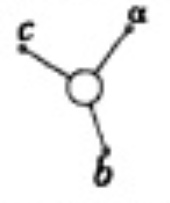
\includegraphics[width=0.1\textwidth]{кругичто}
 \hspace{20pt} 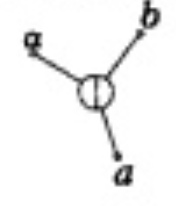
\includegraphics[width=0.1\textwidth]{кругичто1}
\\и т.д. Отрезочки в этих графических представлениях показывают связь пере-
менных с соответствующими формулами. «Склеив» все одноименные точки, мы получим сеть (рис. 1).
Это еще не алгоритм, но уже и не первозданный хаос, не путаница и не сумятица.

\begin{center}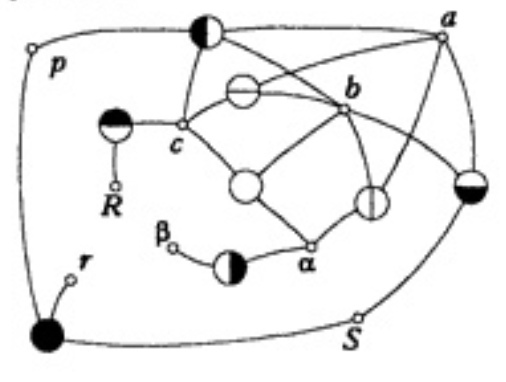
\includegraphics[width=0.25\textwidth]{многокруов} \end{center}
\begin{flushleft}Рис. 1\end{flushleft}

Построенная нами сеть описывает неко- торые свойства прямоугольного треуголь
ника, и пока не ясно, как с ее помощью
решить поставленную задачу (и можно ли вообще это сделать). Формулы мы вспо- минали, как говорится, наобум, и поэтому нет гарантии, что среди них окажутся как раз те, из которых удается построить
нужный нам алгоритм. И все же попробуем. Наша сеть очень напоминает марсианс- кие каналы. Пусть это будет система пустых (незаполненных водой) каналов,
%
точки будут пустыми колодцами, а кру- жочки распределительными станция- ми, которые открывают шлюзы для пуска воды в пустой канал только в том случае,
если во всех остальных каналах, подве денных к данной станции, вода уже есть. Вода в данном случае будет олицетворять наполнение переменных арифметическим содержанием числовым значением.
Итак, что дано в задаче? $а$ и $b$. Пусть в пунктах $a$ и $b$ «забили чистые ключи». По разным каналам вода поступит к распре
делительным станциям 
\includegraphics[width=0.02\textwidth]{круг5},
\includegraphics[width=0.02\textwidth]{круг2},
\includegraphics[width=0.02\textwidth]{круг1},
\includegraphics[width=0.02\textwidth]{круг6},
\includegraphics[width=0.02\textwidth]{круг}, но только три - 
\includegraphics[width=0.02\textwidth]{круг2},
\includegraphics[width=0.02\textwidth]{круг1} и 
\includegraphics[width=0.02\textwidth]{круг6} смогут
открыть шлюзы для наполнения колодцев $c$, $а$, $Ѕ$. В дальнейшем вода из этих колодцев поступит в другие каналы, и шлюзы на втором этапе смогут открыть распределительные станции 
\includegraphics[width=0.02\textwidth]{круг5},
\includegraphics[width=0.02\textwidth]{круг4} и 
\includegraphics[width=0.02\textwidth]{круг3},
наполнив колодцы $р$, $R$. $\beta$. Наконец, на третьем шаге шлюзы откроет распределительная станция 
\includegraphics[width=0.02\textwidth]{круг7} наполнив колодец $r$.
Итак, вывод первый: наша совокуп- ность формул достаточна для того, чтобы решить поставленную задачу: отправля- ясь от известных значений а и ь, мы в конце концов сможем найти значение г. Заметим, что этот вывод мы сделали, не производя вычислений, а только анализи- руя структуру сети.
Представим процесс движения воды в виде схемы (рис. 2).
Эта схема показывает, что и как можно вычислить, пользуясь нашей совокуп ностью формул и отправляясь от извест ных значений в и 6. Здесь бросаются в глаза некоторые лишние «рукава», кото- рые не имеют никакого отношения к зада че. Отправляясь из пункта двигаясь строго вверх, обрежем все участки, кото- рые не используются для вычисления ответа, пока не дойдем до исходных дан- ных задачи. В итоге получим новую схему (рис. 3), которая и представляет искомый
\begin{center}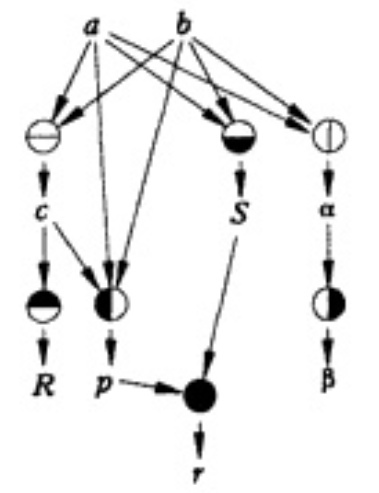
\includegraphics[width=0.25\textwidth]{многокруов1} \end{center}
\begin{flushleft}Рис. 2\end{flushleft}
	\end{multicols}
	\newpage
	\begin{multicols}{3}
		\noindent била повторять: если почти все, кто носит цилиндр, ходят с тросточкой, и вместе с тем почти все, кто ходит с тросточкой, пьют только абсент, то наверняка можно сказать только одно - из тех, кто носит цилиндр, многие пьют только абсент. Многие - да, согласен. А сказать «почти все - это неверно».
		Нечеткие категории - Далеко не един- ственная особенность человеческих рас- суждений. Наитие, догадки, внезапное озарение, «божья искра» столь же при влекательная, сколь и непостижимая тай-
		на за семью печатями.
		-
		Пока еще не удается понять и смодели ровать механизмы ассоциативного мыш- ления, лежащего в основе большинства творческих процессов. В научном тво- рчестве ассоциация проявляется в поиске аналогий, в установлении связей между прототипом и некоторым его образом	
		будет представление о характеризуемом ими понятии. Числовые коэффициенты в ореолах информантов могут выбираться из промежутка (0,1). Если, например, снег «слегка влажный», то можно принять
		
		\begin{center}\textit{снег} = $0,3*$\textit{влажный.} \end{center}
		
		Как же по эталонным ореолам, сообща емым различными информантами, пос- троить обобщенный ореол: понятие$= x_1 *$  понятие$_1$ $+x_2$* понятие$_2$ +...+ $x_n$ понятие$_n$ ? (1)\\ Здесь понятие, понятие, понятие, - совокупность понятий, называемых ниже базисными, которые встречаются в орео лах информантов; $x_1$, $x_2$,\dots,$x_n$ - ко- эффициенты, подлежащие определению. Естественно потребовать, чтобы базис- ное понятие, которое наиболее часто встре чается в сообщаемых информантами
		\columnbreak
	
	\begin{flushright} \hspace*{0.5cm} Представители собачьих\end{flushright}
	\begin{tabular}{ |c|c| } 
		\hline
		Эталон & Ореол  \\ \hline 
		Белый клык & серый  \\ \hline
		Собака & черная,поджарая,  \\
		Баскервилей & глубоко сидящие глаза \\ \hline
		Дружок & одно ухо черное \\ \hline
		Каштанка & рыжая \\ \hline
		Мурзик & белый, мохнатый, \\ 
		& одно ухо черное \\ \hline
		Белый бим  & белый, с рыжими \\  
		Черное ухо & подпалинами одно ухо \\
		&  и одна нога черные \\ \hline
		
	\end{tabular}	
\end{multicols}

		

\end{document}